%------------------------
% Resume Template
% Author : Anubhav Singh
% Github : https://github.com/xprilion
% License : MIT
%------------------------

\documentclass[a4paper,20pt]{article}

\usepackage{latexsym}
\usepackage[empty]{fullpage}
\usepackage{titlesec}
\usepackage{marvosym}
\usepackage[usenames,dvipsnames]{color}
\usepackage{verbatim}
\usepackage{enumitem}
\usepackage[pdftex]{hyperref}
\usepackage{fancyhdr}
\usepackage{gensymb}
\usepackage{pdfpages} 


\pagestyle{fancy}
\fancyhf{} % clear all header and footer fields
\fancyfoot{}
\renewcommand{\headrulewidth}{0pt}
\renewcommand{\footrulewidth}{0pt}

% Adjust margins
\addtolength{\oddsidemargin}{-0.530in}
\addtolength{\evensidemargin}{-0.375in}
\addtolength{\textwidth}{1in}
\addtolength{\topmargin}{-.45in}
\addtolength{\textheight}{1in}

\urlstyle{rm}

\raggedbottom
\raggedright
\setlength{\tabcolsep}{0in}

% Sections formatting
\titleformat{\section}{
  \vspace{-10pt}\scshape\raggedright\large
}{}{0em}{}[\color{black}\titlerule \vspace{-6pt}]

%-------------------------
% Custom commands
\newcommand{\resumeItem}[2]{
  \item\small{
    \textbf{#1}{#2 \vspace{-2pt}}
  }
}

\newcommand{\resumeItemWithoutTitle}[1]{
  \item\small{
    {\vspace{-2pt}}
  }
}

\newcommand{\resumeSubheading}[4]{
  \vspace{-1pt}\item
    \begin{tabular*}{0.97\textwidth}{l@{\extracolsep{\fill}}r}
      \textbf{#1} & #2 \\
      \textit{#3} & \textit{#4} \\
    \end{tabular*}\vspace{-5pt}
}


\newcommand{\resumeSubItem}[2]{\resumeItem{#1}{#2}\vspace{-3pt}}

\renewcommand{\labelitemii}{$\circ$}

\newcommand{\resumeSubHeadingListStart}{\begin{itemize}[leftmargin=*]}
\newcommand{\resumeSubHeadingListEnd}{\end{itemize}}
\newcommand{\resumeItemListStart}{\begin{itemize}}
\newcommand{\resumeItemListEnd}{\end{itemize}\vspace{-5pt}}

%-----------------------------
%%%%%%  CV STARTS HERE  %%%%%%

\begin{document}

%----------HEADING-----------------
%\begin{tabular*}{\textwidth}{l@{\extracolsep{\fill}}r}
 % \textbf{{\LARGE Jeffrey ``Jeff" Anderson}} \\ he/they & \href{mailto:jeffanderson867@ucla.edu}{jeffanderson867@ucla.edu} \\
 % & 404-983-4994
  
  \begin{tabular*}{\textwidth}{l@{\extracolsep{\fill}}r}
    \textbf{{\LARGE Jeffrey ``Jeff" Anderson}} \\  & \href{mailto:jeffanderson867@ucla.edu}{jeffanderson867@ucla.edu} \\
    & 


  
\end{tabular*}
\vspace{-15pt}
%-----------EDUCATION-----------------
\section{Education}
  \resumeSubHeadingListStart
    \resumeSubheading
      {University of California - Los Angeles}{Los Angeles, CA}
      {Bachelor of Science - Mechanical Engineering - GPA: 3.54}{Expected Jun. 2022}
      {\scriptsize{ \footnotesize{\newline{}\textbf{Courses:} 
      Intermediate Fluid Mechanics, Advanced Strength of Materials, Principles of Nanoelectronics, Environmental Nanotechnology
      }}}
    \resumeSubHeadingListEnd
	    
\vspace{-10pt}
%-------------WORK EXPERIENCE-------------
\section{Technical Work Experience}
\resumeSubHeadingListStart
    \resumeSubheading{NanoClear Technologies}{Pasadena, CA}
    {Process Engineer Associate}{May - Sep. 2019, Jun. - Dec. 2020}
    \resumeItemListStart
    	\resumeItem{}{Install and validate semiconductor process equipment including e-beam evaporator and plasma etcher. Direct electrical and process piping contractors in supporting equipment and create standard operating procedures, recipes, and custom fixturing for unique substrates.}
      \resumeItem{}
          {Create custom tooling and support software for environmental materials testing of nano-enabled super-hydrophobic and super-hydophillic surfaces. Port existing processes to new tooling and
applications. Engage rapid-prototyping manufacturers.}
      \resumeItem{}{Substrate Dipping and Drying Robot: Engineer low-cost, user programmable substrate dipping and drying robot on 3D printer platform for production with documentation. Design subject to multi-dicipline review.}
        
	\resumeItem{}{Environmental Chamber: Design environmental chamber for materials
testing. Hold $\pm 0.5 \degree \textsc{C}$ and lower bound $\% \textsc{RH}$ with cycling behavior. Conduct design validation with supporting experimental data. Design requires Raspberry Pi, Arduino, PID control, and python GUI.}
    \resumeItemListEnd

\resumeSubheading{Bruin Racing - Super Mileage}{Los Angeles, CA}
    {Powertrain Lead and Lab Manager}{Sep. 2018 - Pres.}
    \resumeItemListStart
    	\resumeItem{}{Project manage six-person multi-disciplinary team for high-efficiency vehicle powertrain. Establish iterative weight, manufacturing time, and cost reduction metrics subject to design specifications.}
    	\resumeItem{}{Create standard operating procedures and shop layout.}
        \resumeItem{}{Torque Sensing Engine Mount: Coordinate mechanical and electrical team members to sense engine torque output using load cells for real-time engine control unit feedback.}
        \resumeItem{}{Fuel Pressurization: Design pressure vessel and safe regulation for static fuel pressurization. Conduct design safety validation including burst testing.}
        \resumeItemListEnd

\resumeSubHeadingListEnd
%-----------WORK EXPERIENCE-------
\section{General Work Experience}
\resumeSubHeadingListStart
\resumeSubheading{University Cooperative Housing Association}{Los Angeles, CA}
	{Secretary of the Board of Directors} {Nov. 2020 - Pres.}
	\resumeItemListStart
		\resumeItem{}{Direct policy governance in non-profit's mission to provide affordable housing to over 400 UCLA students and mitigate Covid-19 financial losses. Establish advertising campaign efficacy metrics to increase membership.  Seven elected directors and multiple committees.}
    \resumeItemListEnd
\resumeSubheading{California NanoSystems Institute - 
    Integrated Systems Nanofabrication Cleanroom
    }{Los Angeles, CA}
        {Lab Assistant}{Feb. - Jun. 2019}
        \resumeItemListStart
            \resumeItem{}
              {Ensure tools operate within specifications, procure chemicals dispose of waste, maintain cleanroom(particle count, laundry, eg.).
    }
        \resumeItemListEnd
\resumeSubheading{Wellstar Kennestone Hospital}{Marietta, GA}
    {Technician - Advanced Endoscopy Center and Linen Technician}{Jun. - Sep. 2018}
    \resumeItemListStart
        \resumeItem{}
          {Take Vital signs, transport patients between rooms, turnover rooms, conduct inventory, observe infection protocols, distribute linen.}
	%\resumeItem{}{Distributing Linen}
    \resumeItemListEnd
\resumeSubHeadingListEnd

%-----------PROJECTS-----------------
\vspace{-10pt}
\section{Projects}
\resumeSubHeadingListStart
%\resumeSubheading{UCLA Department of Mechanical and Aerospace Engineering}{Los Angeles, CA}{Student}{Sep. 2018 - Pres.}
   % \resumeItemListStart
    	\resumeSubItem{Physicss 4BL: 2D Acoustic Mapper}{: Planar acoustic mapping using omnidirectional microphones and speaker.}
        \resumeSubItem{Engineering 96: Rockets}{: Carbon fiber and 3D printed model rockets(1-3 ft. in length). Suspended egg payload carrier.}
   % \resumeItemListEnd
    

\vspace{2pt}


\vspace{-2pt}
\resumeSubItem{IdeaHacks2020 Hardware Hackathon, Education Category Winner}{: Automatic book reader using vision processing API on Raspberry Pi in under 48 hours. Five-person team.}
\resumeSubItem{IdeaHacks2019 Hardware Hackathon, 1st Place Winner}{: RFID bike lock using CAD, 3-D printers in under 48 hours. Five-person team.}
\resumeSubItem{For Fun}{: ESP32-based Bluetooth keyboard(in progress). Raspberry Pi home VPN, network DNS ad blocking, and 3D printing server, amateur radio.}

%\vspace{2pt}


\vspace{2pt}
\resumeSubHeadingListEnd

\vspace{-10pt}

\section{Skills}
	\resumeSubHeadingListStart
	\resumeSubItem{Languages}{~~~~~~Python, MATLAB, Julia, \LaTeX, Arduino }
	\resumeSubItem{Tools}{~~~~~~~~~~~~~~SolidWorks, Git, Minimal Simulink and KiCAD}
%\resumeSubItem{OS}{~~~~~~~~~~~~~~~~~Linux(Manjaro, Ubuntu), Windows, MacOS}
\resumeSubHeadingListEnd

\vspace{-5pt}


%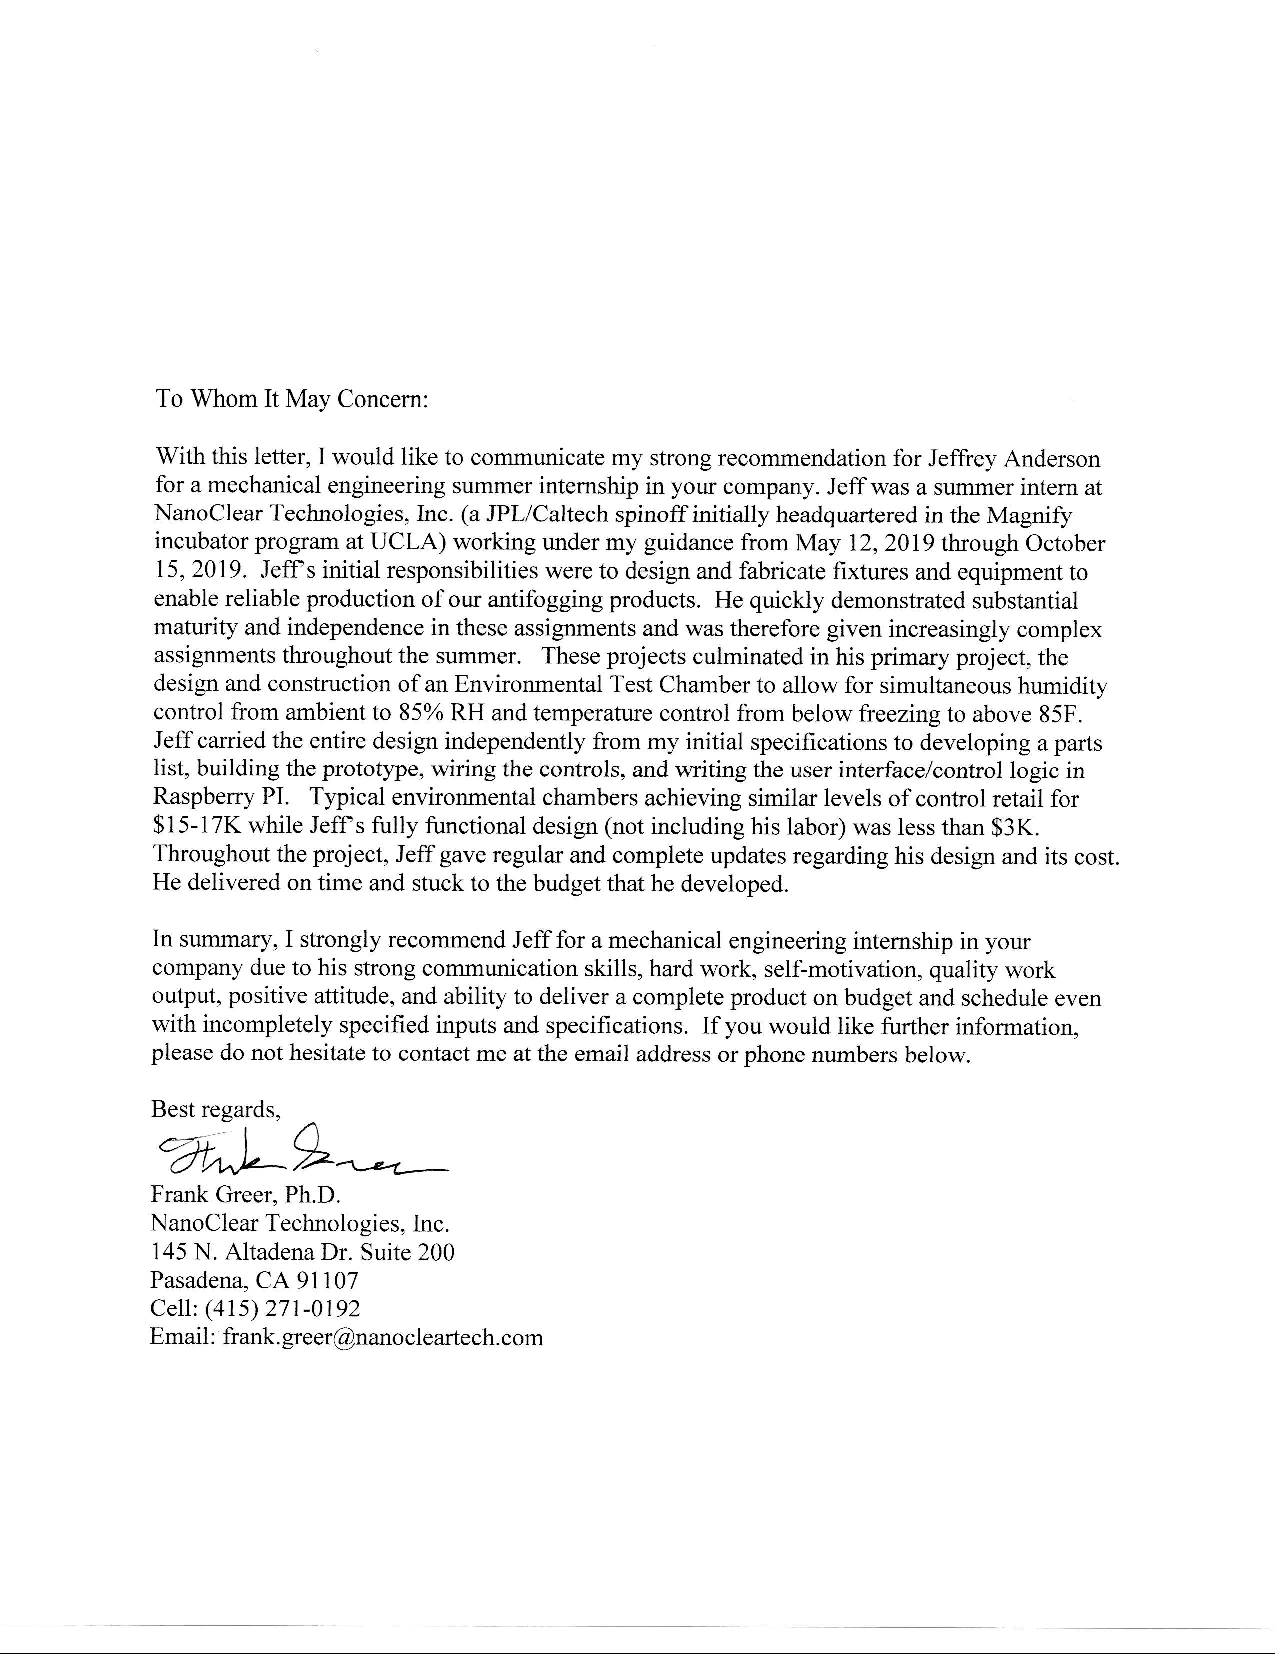
\includepdf[page={1}]{RecommendationLetter-FrankGreer}
\end{document}